
%(BEGIN_QUESTION)
% Copyright 2014, Tony R. Kuphaldt, released under the Creative Commons Attribution License (v 1.0)
% This means you may do almost anything with this work of mine, so long as you give me proper credit

Kretsen som vises her kalles ofte en {\it strømfordeler}. Beregn spenningsfallet over hver motstand, strømmen gjennom hver motstand og den totale resistansen som 9-voltsbatteriet ``ser''.
Regn ut:
\begin{itemize}[noitemsep]
	\item spenningen over hver motstand
	\item strømmen gjennom hver motstand
	\item den totale resistansen som 9-voltsbatteriet ``ser''
\end{itemize}



$$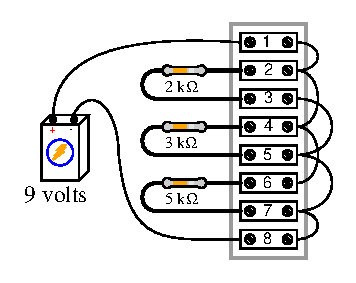
\includegraphics[width=15.5cm]{i01147x01.eps}$$

\begin{itemize}
\item{} Strøm gjennom motstand på 2 k$\Omega$  = 
\item{} Strøm gjennom motstand på 3 k$\Omega$  = 
\item{} Strøm gjennom motstand på 5 k$\Omega$  = 
\item{} Spenning over hver motstand = 
\item{} $R_{total}$ = 
\end{itemize}

\underbar{file i01147}
%(END_QUESTION)





%(BEGIN_ANSWER)

\begin{itemize}
\item{} Strøm gjennom 2 k$\Omega$-motstanden = 4.5 mA
\item{} Strøm gjennom 3 k$\Omega$-motstanden = 3 mA
\item{} Strøm gjennom 5 k$\Omega$-motstanden = 1.8 mA
\item{} Spenning over hver motstand = 9 volt
\item{} $R_{total}$ = 967.74 $\Omega$
\end{itemize}

%(END_ANSWER)





%(BEGIN_NOTES)

Noen elever kan synes diagrammet er vanskelig å følge, og analysen blir da enklere ved å tegne et ekvivalent skjema for kretsen med alle terminalpunkter merket.  Jeg anbefaler at du ikke foreslår denne løsningen med en gang, men heller utfordrer elevene til å finne problemløsningsteknikker selv.  Sannsynligvis vil noen i klassen ha tenkt på dette selv, og effekten av et slikt forslag er ofte større når det kommer fra en medelev enn fra læreren.

Sørg for å stille elevene dette spørsmålet: ``Hvorfor kalles denne typen krets ofte en {\it strømfordeler}?''

%INDEX% Elektronikkrepetisjon: serie- og parallellkretser

%(END_NOTES)

